\documentclass{beamer}
\usepackage[english]{babel}
\usepackage{calc}
\usepackage[absolute,overlay]{textpos}
\mode<presentation>{\usetheme{tud}}



\usepackage{tikz}
\usetikzlibrary{positioning,arrows}

\tikzset{
  block/.style={
    draw,
    rectangle,
    minimum height=1cm,
    minimum width=1cm,
    align=center
  },
  subblock/.style={
    draw,
    rectangle,
    minimum height=.75cm,
    minimum width=1.5cm,
    align=center
  },
  line/.style={->,>=latex},
  LED/.style={draw,circle,append after command={
        [shorten >=\pgflinewidth, shorten <=\pgflinewidth,]
        %(\tikzlastnode.north) edge (\tikzlastnode.south)
        %(\tikzlastnode.east) edge (\tikzlastnode.west)
        }
    },
  dot/.style={draw,circle,minimum size=2mm,inner sep=0pt,outer sep=0pt,fill=black}
}

\usepackage{pifont}% http://ctan.org/pkg/pifont
\newcommand{\cmark}{\ding{51}}%
\newcommand{\xmark}{\ding{55}}%






\title[Mid-term Presentation]{Leveraging VLC for energy }
\subtitle{disaggregation in Smart Buildings}
\institute[TU Delft]{Delft University of Technology}
\author{Johnny Verhoeff}
\date{\today}

% Insert frame before each subsection (requires 2 latex runs)
\AtBeginSubsection[] {
	\begin{frame}<beamer>\frametitle{\titleSubsec}
		\tableofcontents[currentsection,currentsubsection]  % Generation of the Table of Contents
	\end{frame}
}
% Define the title of each inserted pre-subsection frame
\newcommand*\titleSubsec{Next Subsection}
% Define the title of the "Table of Contents" frame
\newcommand*\titleTOC{Outline}

% define a symbol which can be removed if you don't need it
\newcommand{\field}[1]{\mathbb{#1}}
\newcommand{\Zset}{\field{Z}}

\begin{document} {
	% remove the next line if you don't want a background image
	\usebackgroundtemplate{\includegraphics[width=\paperwidth,height=\paperheight]{images/background-titlepage.jpg}}%
	\setbeamertemplate{footline}{\usebeamertemplate*{minimal footline}}
	\frame{\titlepage}
}

\beamertemplatenavigationsymbolsempty
%\setbeamertemplate{navigation symbols}{}

%{\setbeamertemplate{footline}{\usebeamertemplate*{minimal footline}}
%\begin{frame}\frametitle{\titleTOC}
%	\tableofcontents
%\end{frame}
%}

%\section{First Section}
%\subsection{Section 1 - Subsection 1}


	%intro
	\begin{frame}\frametitle{Energy Disaggregation}

		Energy consumption is a most pressing issue.

		\begin{itemize}

			\item To reduce it, understanding the usage of that energy is needed.

			\item Smart-meter can disaggregate the energy usage in a household.

			\item This is done by recognizing the unique signatures of appliances.

		\end{itemize}

		\begin{figure}[t]
			\centering
			\includegraphics[width=0.7\textwidth]{../chapters/introduction-chapters/energy-consumption-house.png}
			%\caption{An example of energy consumption of a household over the course of a day \cite{kolter2011redd}.}
			%\label{fig:energy-consumption-house}
		\end{figure}

		% For example here we can see the aggregated energy from a household during a day.
		% With the different colors it is indicated what appliance is being used at what time.
		% In the blue we can see 'lighting' as a constant consumer but it can not disaggregate which individual lights are on.

	\end{frame}






	\begin{frame}\frametitle{Lighting Energy}

		Individual lights cannot be disaggregated (yet).

		\begin{itemize}

			\item The reason: Lighting does not have a unique signature. %Which HVAC for example does have.

			\item Instead there are many lights with the same signature.

			\item Still important to be able to disaggregate individual lights. % Because it is the third largest power consumer in an average household.

		\end{itemize}


	\end{frame}





	\begin{frame}\frametitle{VLC}

		VLC is a communication method which uses normal lighting to transmit data.

		\begin{itemize}

			\item This data will also propagate through the current draw.

			\item By choosing the data carefully, each light can be identified by its unique current draw.

		\end{itemize}

	\end{frame}






	\begin{frame}\frametitle{Encoding}
		%Easiest way to use VLC is with OOK

		Most common way to use VLC with LEDs, is with On-off keying (OOK).

		\begin{itemize}

			\item LEDs will be turning on and off according to the data.

			\item Binary data is 0 and 1 valued.

			\item Correspondence: 0 $\xrightarrow{}$ LED off, 1 $\xrightarrow{}$ LED on.

		\end{itemize}
	\end{frame}


	\begin{frame}\frametitle{Overview}

		%Smart-meter will measure aggregated current draw of all LEDs.

		\begin{figure}
			\centering
			\resizebox {0.8\textwidth} {!} {
				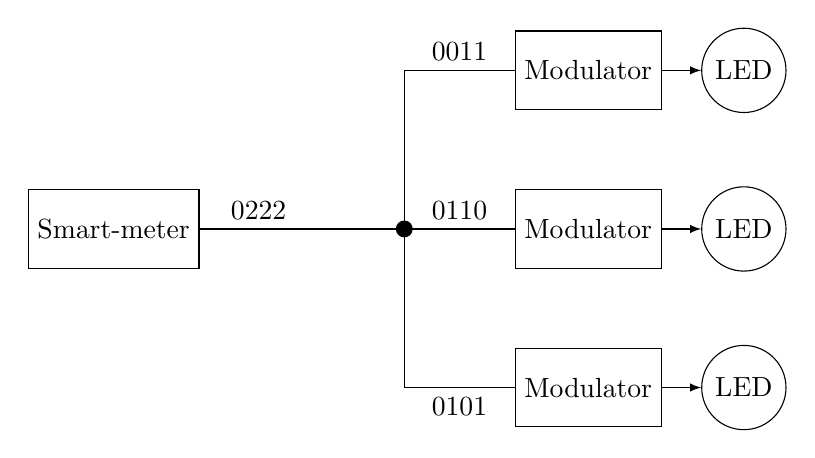
\begin{tikzpicture}

					\node[block] (smart_meter) {Smart-meter};				

					% second mod.
					\node[block, right = 4cm of smart_meter] (second_modulator) {Modulator};
					\node[LED, right = 0.5cm of second_modulator] (second_led) {LED};
					\draw[line] (second_modulator.east) -- (second_led.west) node [midway, right] {};

					% first mod.
					\node[block, above = 1cm of second_modulator] (first_modulator) {Modulator};
					\node[LED, right = 0.5cm of first_modulator] (first_led) {LED};
					\draw[line] (first_modulator.east) -- (first_led.west) node [midway, right] {};

					% third mod.
					\node[block, below = 1cm of second_modulator] (third_modulator) {Modulator};
					\node[LED, right = 0.5cm of third_modulator] (third_led) {LED};
					\draw[line] (third_modulator.east) -- (third_led.west) node [midway, right] {};

					\node[dot, right = 2.5cm of smart_meter] (CP) {};

					\draw (smart_meter.east) -- (CP) node [pos=0.3, above] {0222};

					\draw (CP) |- (first_modulator.west) node  [pos=0.75, above] {0011};
					\draw (CP) |- (second_modulator.west) node [pos=0.75, above] {0110};
					\draw (CP) |- (third_modulator.west) node  [pos=0.75, below] {0101};

				\end{tikzpicture}
			}
		\end{figure}

		\begin{itemize}

			\item What data to use to modulate the LEDs ?

			\item Which hardware to use for the modulator and smart-meter ?

			\item Evaluate the solutions.

		\end{itemize}

	\end{frame}




	\begin{frame}\frametitle{CDMA}
		Metrics to consider of a CDMA sequence:

		\begin{itemize}

			\item Length of the sequence. % each chip of the code has to be transmitted and therefor takes time.

			\item Number of sequences with the same length. % determines scalability of the system.


			\item Correlation: A measure for determining how much a sequence is similar to another sequence.
			\begin{itemize}

				\item Auto-correlation: Should have one peak, to identify a particular sequence. % To determine if a particular LED's signature is in the received signal.

				\item Cross-correlation: Should be as small as possible, to limit the amount of interference. % Determines the interference that the LEDs have on each other. 
				%Too much interference and information gets lost.
			\end{itemize}

		\end{itemize}
	\end{frame}


	\begin{frame}\frametitle{Comparison CDMA Sequences}
		

		% these are the sequences which I have investigated 
		% The orthogonal sequences work really well when the transmitters can be synchronized.
		% But due to the nature of lights, they will transmit a-synchronous.
		% The other sequences work in a-synch circumstances.
		% Where the Gold seq. work slight better and have better scalability.


		\begin{table}
			\centering
			\resizebox {\textwidth} {!} {
				\begin{tabular}{ | l | l | l | l | }

					\hline
															& Orthogonal Seq. 			& PN Seq.						& Gold Seq.				\\ \hline
			Synchronous	Transmission						& \cmark					& \cmark						& \cmark				\\ \hline
			A-synchronous Transmission						& \xmark					& \cmark						& \cmark				\\ \hline
			Peaks auto-correlation (synchronous)			& 1							& 1								& 1						\\ \hline
			Peaks auto-correlation (a-synchronous)			& $> 1$						& 1								& 1						\\ \hline
			Low cross-correlation (synchronous)				& \cmark					& \cmark						& \cmark				\\ \hline
			Low cross-correlation (a-synchronous)			& \xmark					& \cmark						& \cmark				\\ \hline
			Math. bounded cross-correlation (synchronous)	& \cmark					& \xmark						& \cmark				\\ \hline
			Math. bounded cross-correlation (a-synchronous)	& \xmark					& \xmark						& \cmark				\\ \hline
			Scalability ($C \propto L$)						& \cmark					& \xmark						& \cmark				\\ \hline		


				\end{tabular}
			}

		\end{table}
	\end{frame}



	\begin{frame}\frametitle{Mapping Problem}
		CDMA sequences are designed for and used in (wireless) telecommunications.

		\begin{itemize}

			\item Due to the use of analog radio signal the symbols are +1 and -1.

			\item LEDs can have the two state: Off (0) and On (1).

			\item Mapping between these two sets of symbols must take place.

			\item This mapping alters the way the correlation is calculated.

		\end{itemize}
		
	\end{frame}


	\begin{frame}\frametitle{Probabilistic Scheme}
		Cross-correlation is not negligible.

		\begin{itemize}

			\item Cross-correlation is a function of the length of the sequence.

			\item The maximum number of concurrent transmitters $m$ can be calculated, such that no interference will take place. % which will be a function of the length of the sequence.

			\item A probability $p$ is assigned to each transmitter based on the sequence and the time frame and completeness that the user requires.

		\end{itemize}
	\end{frame}


	\begin{frame}\frametitle{Theory To Practice}
		In theory this works.

		
	\end{frame}




	%hardware

	\begin{frame}\frametitle{TITLE}
		DC: use current source per LED for constant and flat current curve, with nice superimposition results
	\end{frame}

	\begin{frame}\frametitle{TITLE}
		AC is not constant, LED require certain amount of voltage
	\end{frame}

	\begin{frame}\frametitle{TITLE}
		Detection circuit for a certain amount of voltage for LEDs and current source for constant and flat current curve, with nice superimposition results
	\end{frame}

	\begin{frame}\frametitle{TITLE}
		DC: use burden resistor with output to adc to measure DC current
	\end{frame}

	\begin{frame}\frametitle{TITLE}
		AC: hall effect too noisy, so also use burden resistor: will produce + and - voltage
	\end{frame}

	\begin{frame}\frametitle{TITLE}
		AC: burden resistor will produce + and - voltage so add half of adc vcc and then to ADC
	\end{frame}




	%cdma

	\begin{frame}\frametitle{TITLE}
		All LEDs are basically transmitters on same freq. and same time.
	\end{frame}

	\begin{frame}\frametitle{TITLE}
		Therefor TDM and FDM are out and CDM is used
	\end{frame}

	\begin{frame}\frametitle{TITLE}
		Concept of correlation: auto and cross
	\end{frame}

	\begin{frame}\frametitle{TITLE}
		Want low cross correlation with all time shifts and high autocorr. at zero time shift and low autocorr at all other time shifts.
	\end{frame}

	\begin{frame}\frametitle{TITLE}
		comparison of orth. pn and gold
	\end{frame}



	% testbed

	\begin{frame}\frametitle{TITLE}
		DC test bed 6 individual LEDs
	\end{frame}

	\begin{frame}\frametitle{TITLE}
		AC test bed 3 individual commercial LEDs
	\end{frame}

	\begin{frame}\frametitle{TITLE}
		Correlation results with contious method DC
	\end{frame}

	\begin{frame}\frametitle{TITLE}
		Correlation results with contious method AC
	\end{frame}





	\begin{frame}\frametitle{TITLE}
		Something with scalabity ??
	\end{frame}


	\begin{frame}\frametitle{TITLE}
		Conclusion ... ? ? 
	\end{frame}











\end{document}
